\chapter{Dados do sistema}
\label{cha:Dados do sistema}

Para satisfazer os requisitos e os casos de uso, foi necessário modelar os dados disponíveis ao sistema e ao algoritmo.

\section{Modelo Entidade-Relacionamento}

A imagem \ref{fig:diagrama-classes} exibe o diagrama do modelo entidade-relacionamento (ER), que descreve os dados no modelos de entidades (coisas de interesse) e seus relacionamentos. O modelo ER segue a notação do Peter Chen \cite{peter-chen}. 

\begin{figure}[ht]
    \begin{center}
    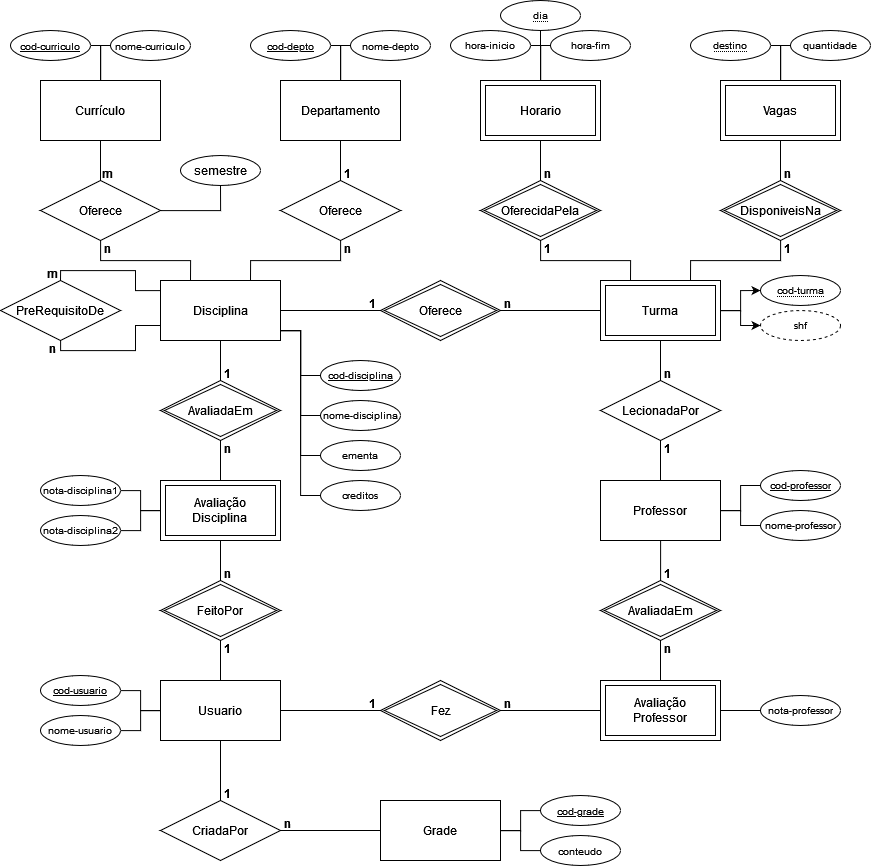
\includegraphics[width=390pt]{figuras/diagrama-er-chen-pdf.png}
    \caption{Diagrama do modelo entidade-relacionamento}
    \label{fig:diagrama-classes}
    \end{center}
\end{figure}

\section{Modelo Físico}

A imagem \ref{fig:modelo-fisico} exibe o diagrama físico dos dados com base no modelo ER. Ele representa a estrutura implementada no banco de dados, com suas tabelas e chaves primárias (PK) e chaves estrangeiras (FK).

\begin{figure}[ht]
    \begin{center}
    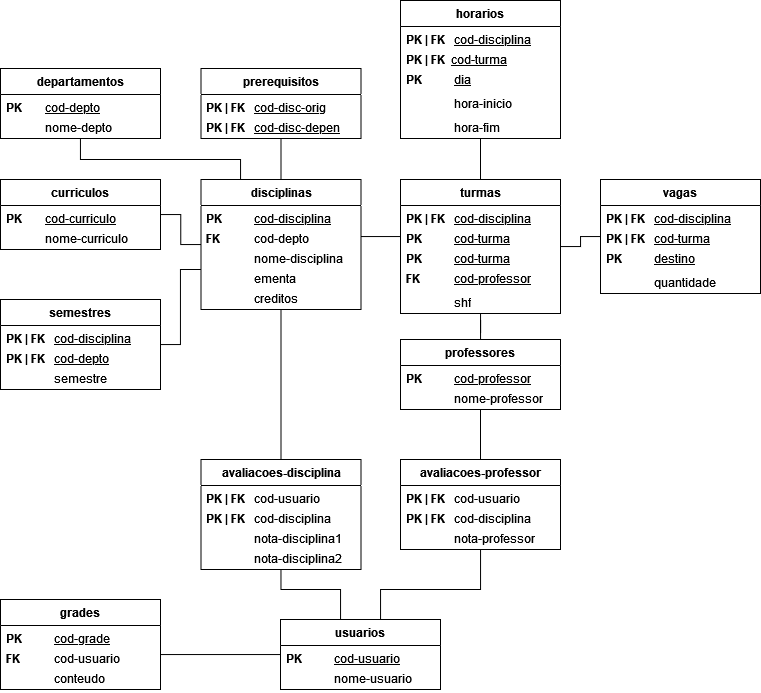
\includegraphics[width=390pt]{figuras/modelo-fisico.png}
    \caption{Diagrama do modelo físico dos dados}
    \label{fig:modelo-fisico}
    \end{center}
\end{figure}

\section{Dicionario de dados}

O dicionario de dados possui a função de categorizar os dados. Ele é uma coleção de metadados do modelo físico. O dicionario de dados está disponível na tabela \ref{tab:dicionario-dados}.

\begin{longtable}{ | >{\raggedright}m{0.2\columnwidth} | >{\raggedright}m{0.4\columnwidth} | >{\raggedright}m{0.1\columnwidth} | >{\raggedright}m{0.2\columnwidth} | }
    \hline\endhead
    % \multicolumn{5}{|c|}{Dicionario de dados}\tabularnewline\hline\hline\endfirsthead
    % \hline\hline
    % \multicolumn{2}{|c|}{Dicionario de dados (continuação)}\tabularnewline\hline\hline\endhead
    % \hline\endfoot
    \hline\caption{Dicionario de dados}\endlastfoot

    \textbf{Coluna} & \textbf{Descrição} & \textbf{Tipo} & \textbf{Domínio}\tabularnewline\hline
     
    cod-curriculo & Identificador do currículo. Exemplo: "eng19.1" & string & Sem restrição.\tabularnewline\hline
    nome-curriculo & Nome curto do currículo. Exemplo: "Engenharia | 19.0". & string & Sem restrição.\tabularnewline\hline
    semestre & Semestre recomendado para cursar a disciplina de acordo com o currículo. & int & Valor entre 1 e 10. Pode ser nulo.\tabularnewline\hline

    cod-depto & Abreviação de três letras do departamento, conforme disponibilizado no microhorario. Exemplo: "ENG". & string & Três letras maiúsculas.\tabularnewline\hline
    nome-depto & Nome do departamento, conforme disponibilizado no microhorario. Exemplo: "Engenharia". & string & Sem restrição.\tabularnewline\hline

    cod-disciplina & Código da disciplina. Exemplo: "INF1011". & string & Três letras maiúsculas seguidas de 4 números.\tabularnewline\hline
    nome-disciplina & Nome da disciplina. Exemplo: "Semântica de Linguagens". & string & Sem restrição.\tabularnewline\hline
    ementa & Ementa da disciplina. & string & Sem restrição. Pode ser nulo.\tabularnewline\hline
    creditos & Quantidade de créditos da disciplina. & int & Valor entre 0 a 30.\tabularnewline\hline

    cod-disc-orig & Código da disciplina que possui algum pré-requisito. & string & Mesmo do cod-disciplina.\tabularnewline\hline
    cod-disc-depen & Código da disciplina que é algum pré-requisito de outra disciplina. & string & Mesmo do cod-disciplina.\tabularnewline\hline

    dia & Dia da semana que a turma é oferecida & string & "seg", "ter", "qua", "qui", "sex" ou "sab".\tabularnewline\hline
    hora-inicio & Hora do inicio da aula da turma & int & Valor entre 7 e 21.\tabularnewline\hline
    hora-fim & Hora do fim da aula da turma & int & Valor entre 9 e 23, deve ser maior que hora-inicio.\tabularnewline\hline
    
    shf & Flag de disciplina "Sem Horário Fixo". & boolean & Sem restrição.\tabularnewline\hline
    destino & Destino das vagas disponíveis. Exemplo: "QQC" (Qualquer curso), "BCO" (Bacharelado em Engenharia de Computação), entre outros. & string & Três letras maiúsculas. Pode ser nulo.\tabularnewline\hline
    quantidade & Quantidade de vagas disponíveis. & int & Valor maior que 0.\tabularnewline\hline

    cod-professor & Código do professor, gerado ao inserir o professor no sistema. & string & Sem restrição.\tabularnewline\hline
    nome-professor & Nome do professor, conforme disponibilizado no microhorário & string & Sem restrição.\tabularnewline\hline

    nota-disciplina1 & Nota da categoria 1 da disciplina avaliada. & int & Valor entre 1 e 5.\tabularnewline\hline
    nota-disciplina2 & Nota da categoria 2 da disciplina avaliada. & int & Valor entre 1 e 5.\tabularnewline\hline
    nota-professor & Nota do professor avaliada. & int & Valor entre 1 e 5.\tabularnewline\hline

    cod-usuario & Código do usuário, representado por sua matrícula & int & 7 números.\tabularnewline\hline
    nome-usuario & Nome do usuário & string & Sem restrição.\tabularnewline\hline

    cod-grade & Código da grade, gerado ao salvar uma nova grade. & string & 8 caracteres em formato base64.\tabularnewline\hline
    conteudo & Conteúdo codificado da grade horária, que é decodificado pela interface ao exibir. & string & Sem restrição.

    \label{tab:dicionario-dados}
\end{longtable}
